\documentclass[11pt,a4paper]{article}
\usepackage[T1]{fontenc}
\usepackage[utf8]{inputenc}
\usepackage[italian]{babel}
\usepackage[a4paper,left=23mm,right=23mm,top=24mm,bottom=23mm]{geometry}
\usepackage{lmodern}
\usepackage{microtype}
\usepackage{xcolor}
\usepackage{graphicx}
\usepackage{tikz}
\usetikzlibrary{arrows.meta}
\usepackage[hidelinks]{hyperref}
\hypersetup{pdftitle={Forza 4},bookmarksnumbered=true}

\definecolor{reportblue}{gray}{0}
\definecolor{reportgray}{gray}{0.35}
\pagestyle{plain}
\emergencystretch=2em
\widowpenalty=10000
\clubpenalty=10000
\setlength{\parindent}{0pt}
\setlength{\parskip}{2.5pt plus 0.5pt minus 0.5pt}
\raggedbottom

\begin{document}
\hypersetup{pageanchor=false}
\begin{titlepage}
\thispagestyle{empty}
\centering
\vspace*{\fill}
{\Huge\bfseries Forza 4\par}
\vspace{12mm}
{\Large Daniele De Blasio\par}
\vspace*{\fill}
\end{titlepage}

\hypersetup{pageanchor=true}
\pagenumbering{roman}
\tableofcontents
\clearpage
\pagenumbering{arabic}

\section{Architettura e responsabilità}

L'applicazione è composta da un server scritto in C e da un client testuale scritto in Python. Il server gestisce lo stato delle partite: riceve le richieste, controlla chi può giocare e di chi è il turno, applica le mosse e stabilisce il risultato. Il client legge i comandi dell'utente e mostra le risposte. In questo modo i client non devono mantenere e sincronizzare due copie della partita. Si possono anche aggiungere altre interfacce lasciando le regole di gioco sul server.

Server e client comunicano tramite socket TCP. TCP mantiene l'ordine dei dati e ne garantisce la consegna finché la connessione funziona: questo è utile perché le mosse devono arrivare nell'ordine corretto. I comandi sono piccoli e vengono scambiati come testo, senza usare WebSocket, HTTP o servizi esterni. Il formato testuale richiede poche dipendenze e permette di leggere direttamente i messaggi scambiati. Convertire una griglia di 42 celle in testo ha un costo trascurabile.

Il server è diviso in cinque moduli. Il modulo game contiene le regole di gioco, senza socket né thread; net riceve le righe e invia i messaggi; state gestisce i client, le partite e i cambiamenti di stato; commands interpreta le richieste; server crea il socket di ascolto e avvia i thread. Gli header condivisi dichiarano le strutture e le funzioni usate dai vari moduli. Questa divisione permette di verificare le regole di gioco senza avviare una connessione di rete.

Nel client un thread legge e invia i comandi, mentre il thread principale riceve i messaggi. Così le notifiche degli altri utenti possono comparire anche mentre l'utente sta scrivendo. Gestire tutto in sequenza richiederebbe una richiesta esplicita per ricevere ogni aggiornamento. Il thread di invio è daemon, quindi non impedisce al client di chiudersi quando il server termina la connessione.

Docker Compose definisce due servizi: server e client. Nella rete Docker il client può raggiungere il server usando il nome del servizio server. Host e porta vengono letti da variabili di ambiente. Le immagini definiscono la famiglia degli strumenti di compilazione e dell'interprete da usare. Il server espone la porta TCP 5555. Ogni client viene avviato in un container interattivo separato, ma tutti usano la stessa immagine.

\begin{figure}[ht]
\centering
\begin{tikzpicture}[
  font=\small,
  box/.style={draw=reportblue, rounded corners=2mm, fill=reportblue!5,
    align=center, minimum height=10mm},
  module/.style={box, text width=39mm, font=\footnotesize},
  connection/.style={draw=reportblue, line width=0.8pt,
    {Latex[length=2mm]}-{Latex[length=2mm]}}
]
\node[box, text width=47mm] (client1) at (-4,0)
  {\textbf{Client Python 1}\\Comandi e visualizzazione};
\node[box, text width=47mm] (client2) at (4,0)
  {\textbf{Client Python 2}\\Comandi e visualizzazione};
\draw[draw=reportblue, rounded corners=2mm, fill=reportblue!2]
  (-7.4,-1.8) rectangle (7.4,-4.65);
\node[font=\small\bfseries, text=reportblue] at (0,-2.15)
  {Server C: un thread per connessione};
\node[module] at (-4.8,-2.85) {\texttt{server}\\Ascolto e avvio thread};
\node[module] at (0,-2.85) {\texttt{net}\\Ricezione e invio};
\node[module] at (4.8,-2.85) {\texttt{commands}\\Lettura dei comandi};
\node[module] at (-2.4,-4) {\texttt{state}\\Client e partite condivisi};
\node[module] at (2.4,-4) {\texttt{game}\\Regole di gioco};
\draw[connection] (client1.south) -- (-4,-1.8);
\draw[connection] (client2.south) -- (4,-1.8);
\node[align=center, font=\footnotesize, text=reportgray] at (0,-1.12)
  {TCP, porta 5555\\Comandi, risposte e notifiche};
\end{tikzpicture}
\caption{Ogni client comunica con lo stesso server. I riquadri interni
mostrano i cinque moduli, non l'ordine delle chiamate.}
\label{fig:architecture}
\end{figure}

\clearpage

\section{Concorrenza e stato condiviso}

\subsection{Thread e sincronizzazione}

Il server crea un thread POSIX per ogni connessione. Ogni thread legge in ordine i comandi del proprio client, mentre client diversi possono essere gestiti contemporaneamente. I thread sono detached: al termine liberano le proprie risorse senza che un altro thread debba attenderli con una join. Non serve recuperarne un risultato e il server può continuare ad accettare utenti. Questa soluzione è adatta a un numero contenuto di connessioni; per migliaia di utenti servirebbe un modo diverso di gestirle.

Le liste dei client e delle partite sono condivise tra i thread. Il mutex globale \texttt{g\_mutex} permette a un solo thread alla volta di eseguire inserimenti, rimozioni, ricerche e cambiamenti di stato. Il controllo che due utenti siano liberi e l'assegnazione della partita avvengono mantenendo lo stesso mutex acquisito. Due richieste \texttt{ACCEPT} contemporanee non possono quindi assegnare allo stesso utente due partite attive.

Ogni client ha anche un mutex per l'invio. Più thread possono mandare notifiche allo stesso destinatario: questo mutex impedisce che i byte di due messaggi si mescolino nel flusso TCP. Quando servono entrambi i mutex, viene acquisito prima quello globale e poi quello di invio. Le funzioni di rete non acquisiscono il mutex globale, quindi non introducono l'ordine inverso.

\subsection{Durata degli oggetti e limiti della concorrenza}

Il flag \texttt{connected} usa un tipo atomico C11, perché viene letto e modificato sia durante l'invio sia durante la pulizia delle sessioni. L'accesso atomico evita accessi concorrenti non protetti a questo flag, ma gli altri campi e la liberazione degli oggetti richiedono ancora il mutex. Dopo aver rilasciato il mutex, non si usa un puntatore a una partita o a un altro client se un altro thread potrebbe modificarlo o eliminarlo. Per inviare errori fuori dalla parte protetta si copiano prima i dati necessari in variabili locali. Anche l'identificativo del nuovo thread viene conservato in una variabile locale: il client potrebbe disconnettersi ed essere liberato prima della chiamata a \texttt{pthread\_detach}.

Per dividere i comandi nei loro argomenti, il parser usa \texttt{strtok\_r} con uno stato separato per ogni riga. La versione \texttt{strtok} può condividere questo stato tra thread e far leggere a un client un argomento di un altro comando. Con \texttt{strtok\_r} ogni connessione viene elaborata in modo indipendente, senza aggiungere un mutex al parser.

Questa gestione dei thread punta alla correttezza e alla semplicità. Diverse notifiche vengono inviate mentre il mutex globale è ancora acquisito. Se un client smette di leggere e il buffer TCP si riempie, può rallentare anche gli altri. Una coda di invio asincrona potrebbe ridurre il problema, ma richiederebbe altri thread, limiti alla coda e regole per stabilire chi gestisce e libera i dati. È un possibile miglioramento: la versione attuale non garantisce di gestire client lenti senza rallentamenti.

\clearpage

\section{Protocollo e rappresentazione dei dati}

\subsection{Formato dei messaggi e comandi}

TCP trasporta una sequenza di byte e non separa i messaggi dell'applicazione. Per questo ogni comando e ogni risposta terminano con un carattere di fine riga. Il server riceve blocchi fino a 4096 byte in un buffer locale al thread e interpreta una riga alla volta. I dati delle righe successive restano nel buffer, evitando una chiamata a \texttt{recv} per ogni carattere. Anche il client conserva i pezzi ricevuti finché trova il fine riga. Una risposta può arrivare con più ricezioni, oppure insieme ad altre risposte: i dati ricevuti non vengono considerati automaticamente un messaggio completo.

La lunghezza delle righe è limitata dal buffer definito da \texttt{MAX\_LINE}. I caratteri CR vengono ignorati, così sono accettati anche i terminatori CRLF. Se una riga supera il limite, la ricezione legge comunque la parte restante senza conservarla: in questo modo non viene scambiata per un nuovo comando. I comandi troppo lunghi restano quindi limitati dal buffer e non permettono di trasmettere quantità arbitrarie di dati.

I comandi sono scritti in maiuscolo e gli argomenti sono separati da spazi. Con \texttt{LOGIN} si associa alla connessione un nickname univoco, di massimo 31 caratteri, composto da lettere, numeri, underscore o trattino. Il nickname serve a riconoscere il giocatore: non ci sono password né controlli sulla sua identità reale. La comunicazione non è cifrata, quindi l'applicazione è pensata per l'uso locale e non come servizio pubblico con account personali.

\newpage

\subsection{Stato delle partite e griglia}

Client e partite sono memorizzati in strutture organizzate in liste collegate. Un contatore, protetto dal mutex, assegna gli identificativi delle partite senza riutilizzarli durante la stessa esecuzione. Per trovare un elemento si scorre la lista: con poche voci questa ricerca è sufficiente e non serve un database. Il tempo di ricerca cresce con il numero di elementi. Partite e identificativi non vengono conservati quando il server viene riavviato.

Ogni partita conserva il proprietario, i partecipanti, il risultato, il turno, le richieste di ingresso e la griglia. Una connessione può possedere più partite in attesa, ma ha un solo puntatore \texttt{active\_game}, quindi può giocare in una sola partita alla volta. Il proprietario sceglie chi ammettere dalla lista delle richieste. Quando accetta un utente, le altre richieste per quella partita vengono eliminate, perché possono giocare soltanto due persone.

La griglia viene inviata come sei righe separate dal carattere slash. Il punto indica una casella vuota, mentre X e O indicano le pedine dei due giocatori. Il client controlla dimensioni e simboli prima di mostrarla. Le risposte sono in italiano, mentre i nomi interni del codice sono in inglese. Gli osservatori ricevono solo le notifiche sullo stato delle partite, senza vedere la griglia o le singole mosse degli altri.


\begin{figure}[ht]
\centering
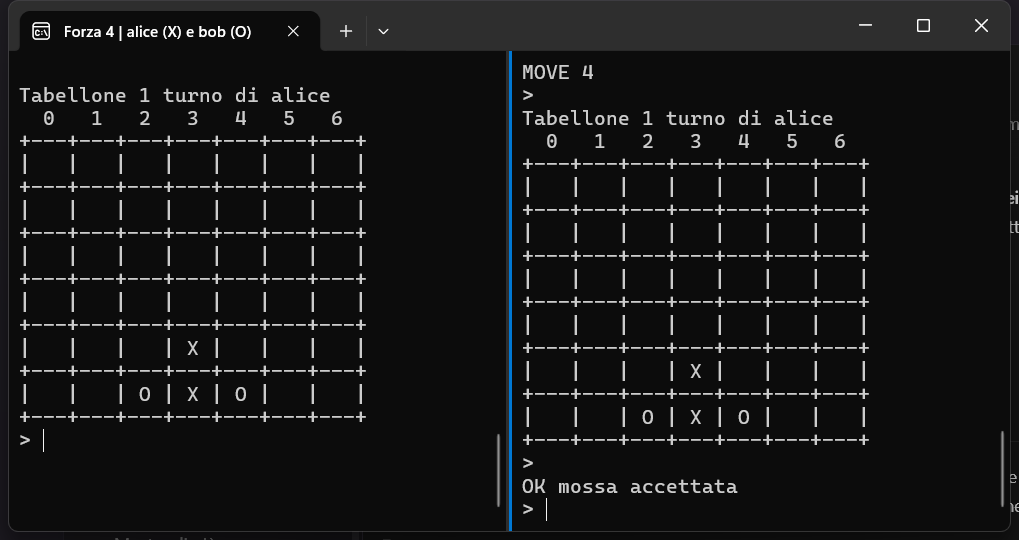
\includegraphics[width=0.94\textwidth,trim=6 6 6 37,clip]{gameplay.png}
\caption{Partita dopo quattro mosse: Alice (X) a sinistra e Bob (O) a destra.
Entrambi vedono la stessa griglia e il turno di Alice.}
\label{fig:terminal-game}
\end{figure}

\clearpage

\section{Regole e transizioni delle partite}

\subsection{Avvio della partita e controllo delle mosse}

Una nuova partita entra subito nello stato \texttt{WAITING}. Non serve uno stato \texttt{CREATED} separato: la partita viene creata e resa disponibile nella stessa operazione atomica, senza attendere un altro evento. Il comando \texttt{JOIN} registra una richiesta di ingresso, ma non avvia il gioco. Solo il proprietario può usare \texttt{ACCEPT}; la partita passa a \texttt{IN\_PROGRESS} se entrambi gli utenti sono ancora liberi.

Il motore di gioco usa una matrice di sei righe e sette colonne e un contatore delle mosse. Per inserire una pedina cerca dal basso la prima cella libera della colonna scelta. Prima di accedere alla matrice controlla gli indici e il numero del giocatore. Se la colonna è piena, la mossa viene rifiutata senza cambiare il turno o il contatore. Il server verifica anche che chi invia la mossa partecipi alla partita e che sia il suo turno.

Per controllare la vittoria si parte dall'ultima pedina e si contano le pedine uguali nei due versi dell'orizzontale, della verticale e delle due diagonali. Non serve controllare tutta la griglia, perché una nuova sequenza vincente deve includere la pedina appena inserita. La vittoria viene controllata prima del pareggio: anche la quarantaduesima mossa può riempire la griglia e allo stesso tempo completare una sequenza di quattro pedine.

\subsection{Conclusione e rivincita}

Quando la partita finisce, lo stato diventa \texttt{FINISHED} e il turno viene azzerato. Il server manda prima la griglia finale ai due partecipanti, indicando il turno con un trattino, e poi il risultato per ciascun giocatore. Gli altri utenti ricevono solo la notifica di fine. Entrambi i giocatori vengono liberati dalla partita attiva. Il comando \texttt{STATE} continua a mostrare soltanto la partita attiva: la griglia finale è già stata inviata, quindi non vengono aggiunti una cronologia o un nuovo significato al comando.

Con \texttt{REMATCH} si può indicare l'identificativo della partita da riaprire. Se viene omesso, viene scelta quella creata più recentemente tra le partite terminate a cui ha partecipato il mittente. Specificare l'identificativo permette di scegliere una partita precisa, senza dipendere dall'ordine della lista. Dopo una vittoria può riaprire la partita solo il vincitore, che ne diventa proprietario; il perdente viene rimosso. La griglia viene svuotata e la partita torna in attesa. Per iniziare servono di nuovo \texttt{JOIN} e \texttt{ACCEPT}: la rivincita non parte automaticamente.

Dopo un pareggio entrambi i giocatori devono confermare la rivincita con \texttt{REMATCH}. La prima conferma avvisa l'altro giocatore e lascia la partita terminata; ripetere il comando non conta come un secondo voto. La seconda conferma viene accettata solo se entrambi sono connessi e non stanno giocando in un'altra partita. La partita torna in attesa con lo stesso proprietario e i vecchi partecipanti vengono rimossi dalla sessione. Le conferme vengono cancellate alla riapertura e quando uno dei giocatori inizia un'altra partita, così un vecchio voto non viene usato per una rivincita successiva.

\begin{figure}[ht]
\centering
\begin{tikzpicture}[
  font=\footnotesize,
  status/.style={draw=reportblue, rounded corners=2mm, fill=reportblue!5,
    text width=30mm, minimum height=13mm, align=center},
  transition/.style={draw=reportblue, line width=0.8pt,
    -{Latex[length=2mm]}}
]
\node[status] (waiting) at (0,0) {\texttt{WAITING}\\In attesa};
\node[status] (playing) at (5.4,0) {\texttt{IN\_PROGRESS}\\In corso};
\node[status] (finished) at (10.8,0) {\texttt{FINISHED}\\Terminata};
\draw[transition] (waiting.east) -- node[above, align=center]
  {\texttt{ACCEPT}\\Utenti liberi} (playing.west);
\draw[transition] (playing.east) -- node[above, align=center, font=\scriptsize]
  {Vittoria o\\pareggio} node[below, align=center, font=\scriptsize]
  {Abbandono o\\disconnessione} (finished.west);
\draw[transition] (finished.south) -- (10.8,-1.65) --
  node[below, align=center, text width=112mm]
  {\texttt{REMATCH}: richiesta del vincitore o consenso di entrambi dopo un pareggio.\\
   La partita torna in attesa, con griglia vuota.}
  (0,-1.65) -- (waiting.south);
\end{tikzpicture}
\caption{Cambiamenti di stato della partita. \texttt{CREATE} la crea in
\texttt{WAITING}; \texttt{JOIN} registra una richiesta senza cambiare stato.
Le condizioni della rivincita sono descritte nel testo.}
\label{fig:game-states}
\end{figure}

\clearpage

\section{Disconnessioni, memoria e limiti}

La ricezione rileva la disconnessione quando l'altro lato chiude il flusso o il socket restituisce un errore. L'invio gestisce anche il caso in cui vengano scritti solo alcuni byte del messaggio e riprova se un segnale lo interrompe. Nel container Linux usa \texttt{MSG\_NOSIGNAL}: scrivere su un socket chiuso restituisce un errore gestibile, invece di terminare il processo con \texttt{SIGPIPE}. Se l'invio fallisce, la connessione viene segnata come chiusa e \texttt{shutdown} sblocca l'eventuale ricezione in attesa.

Il thread del client esegue la pulizia mantenendo acquisito il mutex globale. Elimina le richieste in attesa, termina la partita attiva dando la vittoria all'avversario e cancella le partite in attesa di proprietà dell'utente. Prima di liberare il client, rimuove i suoi riferimenti dalle partite terminate. Infine chiude il socket, distrugge il mutex di invio e libera la struttura del client. In questo modo non restano puntatori a una connessione che non esiste più.

Le strutture delle partite vengono allocate dinamicamente. Le partite terminate restano nella lista perché servono ai comandi \texttt{LIST} e \texttt{REMATCH}. Le richieste vengono invece liberate quando sono accettate, rifiutate o annullate, oppure quando la partita viene ripristinata. Se il server resta in esecuzione a lungo, conservare tutte le partite concluse fa aumentare la memoria usata. Non ci sono un archivio, una cancellazione periodica o un limite complessivo alle partite create.

Lo stato delle sessioni viene conservato solo in memoria. Quando il server si ferma, partite, identificativi e nickname vengono persi. Non sono previsti il recupero delle sessioni dopo un riavvio, la riconnessione automatica o il trasferimento di una partita a un nuovo processo. Se un giocatore si disconnette durante il gioco, la partita termina e non viene sospesa.

Il server controlla nickname, identificativi, colonne, proprietario e turno. Per convertire i numeri usa \texttt{strtol} e controlla overflow, fine della stringa e intervallo prima di convertirli in \texttt{int}. Un numero troppo grande viene rifiutato, senza essere trasformato in una colonna o in un identificativo valido. Questi controlli non forniscono autenticazione forte, non limitano il numero di richieste inviate e non isolano utenti che cercano di disturbare il servizio. La compilazione e i test di regressione verificano i casi eseguiti, ma non dimostrano l'assenza di errori in ogni possibile ordine di esecuzione dei thread.

Il server viene eseguito nell'ambiente Linux delle immagini Docker. Usa thread POSIX e \texttt{MSG\_NOSIGNAL}, senza versioni alternative basate sulle API native di Windows. La compilazione usa C11 e le opzioni -Wall, -Wextra, -Wpedantic e -Werror. Il Makefile include tutti gli header condivisi tra le dipendenze, quindi una modifica alle strutture fa ricompilare il codice.

\clearpage

\section{Strategia di verifica}

I test controllano separatamente le varie parti dell'applicazione. Il motore di gioco viene compilato insieme a un programma di test C che verifica gravità, colonne piene, parametri non validi, vittorie nelle quattro direzioni per entrambi i giocatori, pareggio e ripristino. Un secondo test C chiude un lato di una coppia di socket e scrive sull'altro, per controllare che l'errore non termini il processo. AddressSanitizer e UndefinedBehaviorSanitizer aiutano a trovare errori di memoria e comportamenti non definiti dal linguaggio nei casi eseguiti. Non sostituiscono però l'analisi degli accessi concorrenti tra thread.

Il test di rete controlla anche righe spezzate o ricevute insieme, terminatori CRLF, righe vuote e troppo lunghe, chiusure a metà riga ed errori di ricezione. Conta le chiamate a \texttt{recv} per verificare che più righe già nel buffer non richiedano altre letture dal socket.

I test del protocollo si collegano al server con client TCP e confrontano le risposte con lo stato atteso. Controllano più partite contemporanee, le notifiche a giocatori e osservatori, i risultati, la griglia finale, il cambio di proprietario dopo una vittoria e le due conferme distinte dopo un pareggio. I casi di errore verificano anche che una mossa rifiutata non consumi il turno e che un utente non venga assegnato a due partite attive. Numeri troppo grandi e argomenti con caratteri residui devono produrre un errore senza cambiare griglia o turno.

Una prova invia più login contemporaneamente e confronta il nickname richiesto da ogni socket con quello confermato dal server. Serve a verificare che gli argomenti delle richieste non si mescolino. Altri test controllano le chiusure improvvise e le richieste contemporanee durante la fine delle partite. Le prove usano un container isolato con una porta locale assegnata da Docker. Il container viene rimosso anche se un test fallisce.

La sintassi del client Python viene controllata nella sua immagine Docker. Prima delle prove viene verificata la configurazione Compose e vengono costruite le immagini. Il \texttt{README} spiega come avviare l'applicazione e usare il protocollo.

\end{document}
